\def\year{2019}\relax
\documentclass[letterpaper]{article}
\usepackage{aaai19}
\usepackage{times}
\usepackage{helvet}
\usepackage{courier}
\usepackage{graphicx}
\frenchspacing
\setlength{\pdfpagewidth}{8.5in}
\setlength{\pdfpageheight}{11in}
\setcounter{secnumdepth}{2}

\usepackage[utf8]{inputenc} % allow utf-8 input
\usepackage[T1]{fontenc}    % use 8-bit T1 fonts
\usepackage{url}            % simple URL typesetting
\usepackage{booktabs}       % professional-quality tables
\usepackage{amsfonts}       % blackboard math symbols

\newcommand{\citet}[1]{\citeauthor{#1} ̃\shortcite{#1}}
\newcommand{\citep}{\cite}
\newcommand{\citealp}[1]{\citeauthor{#1} ̃\citeyear{#1}}

\usepackage{upgreek}
\usepackage{amsmath}
\usepackage{soul}
\usepackage{algorithm}
\usepackage{algpseudocode}
\usepackage{booktabs}

\newcommand{\vect}[1]{\vec{#1}}
\DeclareMathOperator{\Feat2Vec}{Feat2Vec}
\DeclareMathOperator{\Word2Vec}{Word2Vec}
\DeclareMathOperator{\Doc2Vec}{Doc2Vec}
\DeclareMathOperator{\q}{{\mathcal{Q}}}
\newcommand{\dotp}{\boldsymbol{\cdot} }
\usepackage{subcaption}

\newcommand{\algojose}{Structured Deep-Out Factorization Machine}
\newcommand{\algoralph}{$\Feat2Vec$}
\usepackage{amssymb}
\usepackage[weather]{ifsym}
\usepackage{amsmath}
\usepackage{upgreek}
\usepackage{bm}
\usepackage{mathtools}
\newcommand{\algoralphabbr}{$\Feat2Vec$}
%
%
\pdfinfo{
/Title (Beyond Word Embeddings: Dense Representations for Multi-modal Data)
/Author (Luis Armona, Ralph Edezath, Jos\'e P. Gonz\'alez-Brenes)
}

\title{Beyond Word Embeddings: Dense Representations for Multi-modal Data}

\author{
  Luis Armona\textsuperscript{\rm1,\rm 2}, Ralph Edezhath\textsuperscript{\rm 2},  Jos\'e P. Gonz\'alez-Brenes,\textsuperscript{\rm 2} \\
  \textsuperscript{\rm 1}Department of Economics, Stanford University, \\
  \textsuperscript{\rm 2}Chegg, Inc.\\
  larmona@stanford.edu, \{redezhath, jgonzalez\}@chegg.com
}

\begin{document}
\maketitle
\begin{abstract}
Methods that calculate dense vector representations for text have proven to be very successful for knowledge representation.
We study how to estimate dense representations for multi-modal data (e.g., text, continuous, categorical).
We propose Feat2Vec as a novel model that supports supervised learning when explicit labels are available, and self-supervised learning when there are no labels.
Feat2Vec calculates embeddings for data with multiple feature types, enforcing that all embeddings exist in a common space.
We believe that we are the first to propose a method for learning self-supervised embeddings that leverage the structure of multiple feature types.
Our experiments suggest that Feat2Vec outperforms previously published methods, and that it may be useful for avoiding the cold-start problem.
\end{abstract}



\section{Introduction}

Informally, in machine learning a \textit{dense representation}, or \textit{embedding}  of a vector   $\vect{x} \in \mathbb{R}^n$  is another vector $\vect{\beta} \in \mathbb{R}^r$ that has much lower dimensionality ($r \ll n$) than the original representation.
In general, we consider two kind of models that produce embeddings:
\textbf{(i)~supervised methods}, like matrix factorization, calculate embeddings that are highly tuned to a prediction task.
For example, in the Nextflix challenge, movie identifiers  are embedded to predict user ratings.
On the other hand, \textbf{(ii)~self-supervised methods} (sometimes referred to as unsupervised methods) are not tuned for the prediction task they are ultimately used for.
For example, word embedding algorithms such as $\Word2Vec$~\cite{mikolov2013distributed} are self-supervised. These algorithms are typically evaluated by analogy solving, or sentiment analysis~\cite{le2014distributed}, even though their loss functions are not tuned for either of these tasks.

Throughout this paper, we refer to any data that has different types of information as multi-modal.
We propose $\Feat2Vec$ as a novel method that  embeds multi-modal data, such as text, images, numerical or categorical data, in a common vector space---for both supervised and self-supervised scenarios.
We believe that this is the first self-supervised algorithm that is able to calculate embeddings from data with multiple feature types.
Consider the non-trivial work that was required to extend a model like Word2Vec to support  additional features.
The authors of the seminal Doc2Vec~\cite{le2014distributed} paper needed to design both a new neural network and a new sampling strategy  to add a single feature (document ID).
$\Feat2Vec$ is a general method that allows calculating embeddings for any number of features.

\section{Feat2Vec}
\label{sec:methods}
In this section we describe how $\Feat2Vec$  learns embeddings of feature groups.

\subsection{Model}
\label{sec:algoralph}
$\Feat2Vec$ operates on multi-modal data that naturally group into different types.
For example, we may group individual words into a single ``text'' feature group;
or we may group individual pixels into a single ``image'' feature group.
We define an entity to be a particular value or realization of a feature group.

$\Feat2Vec$ predicts  a target output  $\hat y$ from a list of feature groups, constructed from a partition $\vect{\pmb{\upkappa}}$ of raw features ${\vect{\mathbf x}}$:
\begin{align}
  {\vect{\mathbf x}} =   \langle \vect{x}_{\vect \upkappa_1}, \vect{x}_{\vect \upkappa_2}, \dots, \vect{x}_{\vect \upkappa_n} \rangle  = \langle \vect{g}_1, \vect{g}_2, \dots, \vect{g}_n \rangle
 \end{align}
Each of the $n$ feature groups  $\vect{g}_i$ is defined a priori by $\vect \upkappa_i$, which indexes the dimensions in ${\vect{\mathbf x}}$  that belong to the $i$-th group.
The number of dimensions of each group may vary, but all of the feature groups are embedded to the same space via their \textit{feature extraction function} $\phi_i$.
A feature extraction function $\phi_i$ acts on the features in $\upkappa_i$. Other features interact with $\vect{x}_{\vect \upkappa_i}$ only via the output of $\phi_i$.
These functions learn how to transform each input (feature group) into an $r$-dimensional embedding in $\mathbb{R}^r$.
More formally, we define our model for a target $y$ as follows:

\begin{align}
\hat y(\vect{\mathbf{x}\vphantom{phi}},\vec{\pmb{\phi}}, \vect{\pmb{\upkappa}\vphantom{phi}} ) = \omega \biggl(
                       \sum_{i =1}^n \sum_{j=i}^n  \overbracket {\phi_i( \vect{x}_{\vect{\upkappa}_i}) }^{ \mathclap  { \text{group $i$}\atop \text{embedding}}} \dotp \overbracket {\phi_j( \vect{x}_{\vect{\upkappa}_j}) }^{ \mathclap  { \text{group $j$}\atop \text{embedding}}}
  \biggr)
 \label{eq:deepfm}
\end{align}

Here, $\omega$ is an activation function.
Intuitively, the dot product ($\dotp$) returns a scalar that measures the (dis)similarity between the embeddings of the feature groups.
A simple  implementation of $\phi_i$ is a linear fully-connected layer, where the output of the $r$-th entry is:
\begin{equation}
\label{eq:fully_connected}
\phi_{i,r}\bigl( \vect{x\vphantom{\theta}}_i; \vect{\uptheta}_r\bigr )_r= \sum_{a=1}^{d_i}  \theta_{r_a} x_{i_a}
\end{equation}
where $ \vect{\uptheta}_r $ are learned weights. Other functional forms of $\phi_i$ we have explored in our experiments include:
\begin{itemize}
\item A convolutional neural network that transforms a text sequence into an $r$-dimensional embedding. This function is able to preserve information in the order of a text sequence, unlike other methods for transforming text to numerical values such as bag-of-words.
\item A deep, fully connected neural network that projects a scalar, such as average rating, into an $r$-dimensional embedding space. This extraction function, by treating the input as numerical instead of categorical, requires inputs close in value (e.g. 4.01 and 4.02 star rating) to have similar embeddings.
\end{itemize}
Any neural function that outputs an $r$-dimensional vector could be plugged into our framework as an extraction function $\phi$.
Although in this work we have only used datasets with natural language, categorical and numerical features, it would be straightforward to incorporate other types of data--e.g. images or audio--with the appropriate feature extraction functions, enabling the embedding of multi-modal features in the same space.

Figure~\ref{fig:architecture} compares existing factorization methods  with our novel model.
Figure~\ref{fig:factorization_machine} shows a Factorization Machine~\cite{rendle2010factorization} that embeds each feature.
Figure~\ref{fig:feat2vec}  shows $\Feat2Vec$ with two feature groups:
the first group only has a single feature which is projected to an embedding (just like matrix factorization);
but the second group has multiple features, which are together projected to a single embedding.
Figure~\ref{fig:neural} shows an approach of using neural networks within factorization machines  that has been proposed multiple times~\cite{DBLP:journals/corr/DziugaiteR15,guo2017deepfm}.
It replaces the dot product of factors with a learned neural function, which has been shown to improve predictive accuracy.
The caveat of this architecture is that is no longer  possible to interpret the embeddings as latent factors related to the target task.

\begin{figure*}[th]
    \centering
    \begin{subfigure}[t]{0.26\textwidth}
        \centering
        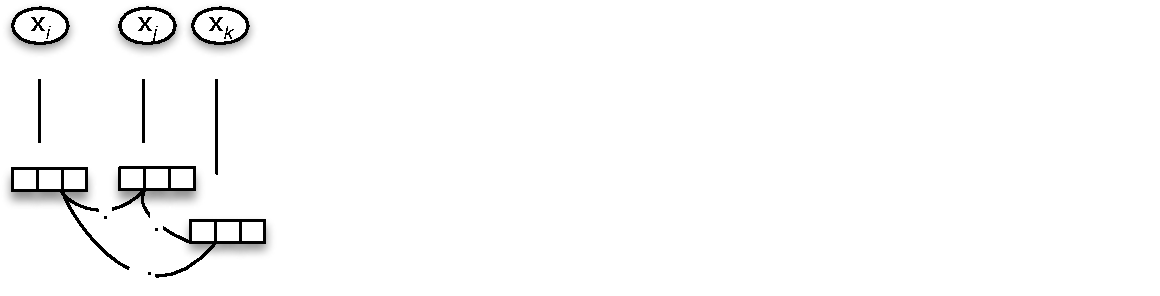
\includegraphics[width=.55\textwidth]{img/diagram_mf.pdf}
        %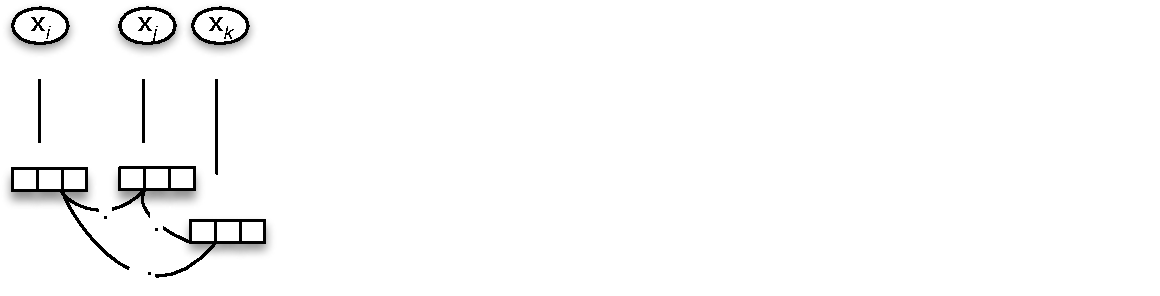
\includegraphics[height=1in]{img/diagram_mf.pdf}
        \caption{\textbf{Factorization Machine}\label{fig:factorization_machine}}
    \end{subfigure}%
    ~
    \begin{subfigure}[t]{0.26\textwidth}
        \centering
        
\includegraphics[width=.5\textwidth]{img/diagram_in.pdf}
        \caption{\textbf{Feat2Vec} \label{fig:feat2vec}}
    \end{subfigure}
    ~
    \begin{subfigure}[t]{0.26\textwidth}
        \centering
        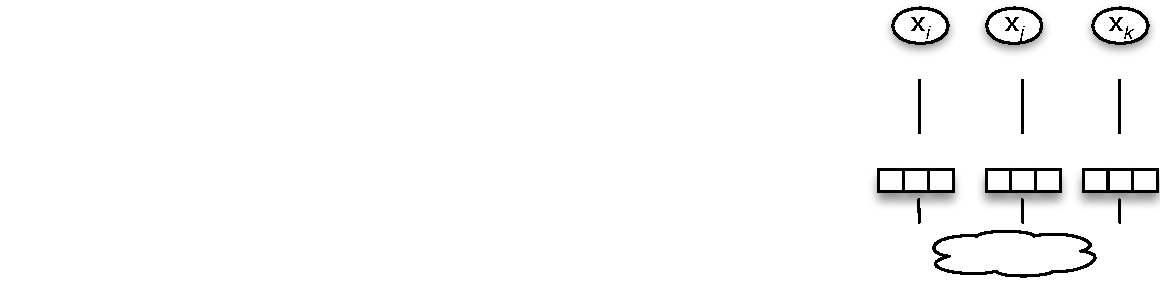
\includegraphics[width=.6\textwidth]{img/diagram_nmf.pdf}
        \caption{\textbf{``Neural"} \label{fig:neural}}
    \end{subfigure}
    \caption{\textbf{Network architectures for factorization models}.  The  white clouds (\Cloud) represent deep layers, for example a convolutional network for text features, while the dots ($\cdot$) denote dot products.
    \label{fig:architecture}
    }
\end{figure*}


Our work in $\Feat2Vec$  significantly expands previously published models.
For example, Principal Component Analysis (PCA) is a common method to learn embeddings of individual dimensions of  data.
Although structured regularization techniques exist~\cite{jenatton2010structured}, it is not obvious how to combine different dimensions in PCA when we are interested in treating a subset of dimensions as a single group, such as words in an item's description.
In traditional factorization methods, item identifiers are embedded and thus need to be observed during training (i.e., cold-start problem).
$\Feat2Vec$ can learn an embedding from an alternative characterization of an item, such as a textual description.
$\Feat2Vec$ extends Factorization Machine~\cite{rendle2010factorization}, in that we allow calculating embeddings for feature groups and we use feature extraction functions.
StarSpace~\cite{wu2017starspace}  introduces feature groups (called entities in their paper), but constrains  them to be ``bags of features,'' is supervised, and limited to two feature types.
In contrast, $\Feat2Vec$ allows continuous features, and does not require the user to assign one feature as a specific target. Additionally, we propose a self-supervised learning algorithm.


\subsection{Supervised Learning from Data}
\label{sec:learning_supervised}

We can learn the the parameters of a Feat2Vec model $ \bm\uptheta$ using training data by minimizing a loss function $\mathcal L$:
\label{sec:learning}
\begin{equation}
\arg \min_{\vect{\uptheta}} \sum_x  \mathcal{L}\bigl(  y(x), \hat y(x;\vect{\uptheta})\bigr)
%+ \gamma||  \bm{\uptheta}||^{w}
\label{eq:learning}
\end{equation}
Here, $y(x)$  is the true target value for $x$ obtained from training data, and $\hat{y}(x)$ is the one estimated by the model (Equation \ref{eq:deepfm});
$\bm\uptheta$ represents the parameters learned in during training (i.e. the parameters associated with the extraction functions $\phi_i$).
%The hyperparameter $\gamma$ controls the amount of regularization.
For labeling and classification tasks, we optimize the binary cross-entropy.

It is straightforward to optimize Equation~\ref{eq:learning} directly.
Typically, this loss will be for a prediction task, and involve at least two feature groups---one of the feature groups is the target label that we want to predict, such as rating, and the other group(s) is the input from which we want to make the prediction, such as review text.

Consider a target feature group $g_i$ that exists in a high dimensional space.
This could be a one-hot encoding of a categorical variable with a large number of possible values.
In such a scenario, it is overwhelmingly costly to feed the model all possible negative labels.
In these cases, we may instead use a binary classifier with implicit sampling~\cite{samplingnotes}.
In implicit sampling, instead of using all of the possible negative labels, one simply samples a fixed number ($k$) from the set of possible negative labels for each positively labelled record.

\subsection{Self-Supervised Learning From Data}
\label{sec:sampling}

We now discuss how $\Feat2Vec$ can be used to learn embeddings in an self-supervised setting with no explicit target for prediction.


The training dataset for a $\Feat2Vec$ model consists of the observed data.
In natural language, these would be documents written by humans, along with document metadata.
Since self-supervised Feat2Vec will require positive and negative examples during training, we supply unobserved data as negative examples.
This sampling procedure is analogous to the $\Word2Vec$ algorithm, which samples a negative observation from a noise distribution $\q_{w2v}$ that is proportional to the empirical frequency of a word in the training data.
Unlike $\Word2Vec$, we do not constrain features types to be words.
Instead, by grouping features using the hyperparameter $\vect{\pmb{\upkappa}}$ in Equation \ref{eq:deepfm}, the model can reason on more abstract entities in the data.
For example, in our experiments on a movie dataset, we define a ``genre'' feature group, where we  group non-mutually exclusive indicators for movie genres, including comedy, action, and drama films.

We start with a dataset $S^+ $ of records with $n$ feature groups.
For each positive (observed) record, we generate $k$ negative labels using the 2-step algorithm documented in Algorithm \ref{algo:samp}.

\begin{algorithm}[htb]
 \caption{Implicit sampling algorithm for self-supervised $\Feat2Vec$}
 \label{algo:samp}
\begin{algorithmic}[1]
\footnotesize
\Function{Feat2Vec\_Sample}{$S^+, k, \alpha_1, \alpha_2$}
\State $S^-  \leftarrow \emptyset $
\For {$\vect{x}^{\,+} \in S^+ $}
	\State Draw a random feature group $\upkappa_i  \sim \q_1(\{\operatorname{params}(\phi_i)\}_{i=1}^{|\vect{\upkappa}|},\alpha_1) $
	\For {$j \in \{1,\ldots,k\}$}
			\State $\vect{x}^{\,-}  \leftarrow \vect{x}^{\,+} $ \Comment  set initially to be equal to the \begin{flushright}positive sample\end{flushright}
			\State Draw a random entity  $\tilde x \sim \q_2(\mathrm{X}_{ \upkappa_i },\alpha_2)$
			\State $\vect{x}^{\,-}_{\upkappa_i}  \leftarrow \tilde x$ \Comment{substitute the $i$-th feature group \begin{flushright}with the sampled one\end{flushright}}
			\State  $S^-  \leftarrow S^-  + \{  \vect{x}^{\,-} \}$
	\EndFor
\EndFor
\State \Return $S^-$
\EndFunction
\end{algorithmic}
\end{algorithm}


Explained in words, our negative sampling method for self-supervised learning iterates over all of the observations of the training dataset.
For each observation $\vect{x}^{\,+}$, it randomly selects the $i$-th feature group from a noise distribution $\q_1(\cdot)$.
Then,  it creates a negative observation that is identical to $\vect{x}^{\,+}$, except that its $i$-th feature group value is replaced by a value sampled from a noise distribution $\q_2(\cdot)$.
In our application, we use the same class of noise distributions (flattened multinomial) for both levels of sampling, but this need not be the case.
We now describe the noise distributions that we use.
Let  $P_{\q}(x)$ denote the probability of $x$ under distribution $\q$.

\textbf{Sampling Feature Groups.} The function $\operatorname{params}$ calculates the complexity of a  feature extraction function $\phi_i$.
To sample a feature group, we choose a feature group $\upkappa_i$ from a multinomial distribution with probabilities proportional to a feature's complexity.
By complexity, we mean the number of parameters we learn that are associated with a feature group's extraction function $\phi_i$.
This sampling procedure places more weight on features that have more parameters and thus are going to require more training iterations to properly learn. The sampling probabilities of each feature group are:

\begin{equation}
P_{\q_1}(\upkappa_i|\operatorname{params}(\phi_i)\}_{i=1}^{|\vect{\upkappa}|},\alpha_1 )  \
= \frac{\operatorname{params}(\phi_i)^{\alpha_1}}{\sum_{j=1}^{|\vect{\upkappa}|} \operatorname{params}(\phi_j)^{\alpha_1}}
\end{equation}
For categorical variables using a linear fully-connected layer, the complexity is simply proportional to the number of categories in the feature group.
However, if we have multiple intermediate layers for some feature extraction functions (e.g., convolutional layers), these parameters should also be counted towards a feature group's complexity.
The hyper-parameter $\alpha_1 \in [0,1]$ flattens the distribution.
 When  $\alpha_1=0$, the feature groups are sampled uniformly,
 and when $\alpha_1=1$, they are sampled exactly proportional to their complexity.


\textbf{Sampling Feature Group Values.}
To sample an entity within a feature group $\upkappa_i$, we use a similar strategy to $\Word2Vec$ and use the empirical distribution of values:
%For  $\q_2(\mathrm{X}_{\upkappa_i}, \alpha_2)$, is the ``flattened'' empirical multionomial distribution over the frequency of the feature values of feature $\upkappa_i$, as in the negative sampling procedure used in $\Word2Vec$ :
\begin{equation}
P_{\q_2}(x|\mathrm{X}_{\upkappa_i},\alpha_2)  \
= \frac{ \operatorname{count}(x)^{\alpha_2}}{\sum_{x_{\upkappa_i}' \in S^+ } \operatorname{count}(x_{\upkappa_i}')^{\alpha_2}}, \quad \alpha_2 \in [0,1]
\end{equation}
Here, $\operatorname{count}(x)$ is the number of times a value $x$ of feature group $i$ appeared in the training dataset $S^+$ , and $\alpha_2$ is again a flattening hyperparameter.


This method will sometimes by chance generate negatively labeled samples that \textit{do} exist in our sample of observed records.
The literature offers two solutions:
in the Negative Sampling of $\Word2Vec$, duplicate negative samples are ignored~\cite{samplingnotes}.
Instead, we account for the probability of random negative labels being identical to positively labeled data using \textit{Noise Contrastive Estimation} (NCE)~\cite{nce}.

%%%%%%%%%%%%%%%%
\subsubsection{The Loss Function for Self-Supervised Learning}
\label{sec:learning}
For our self-supervised learning of embeddings, we optimize a NCE loss function. We adjust the structural statistical model
$\hat y = p(y=1|\vect{x},\vect{\phi}, \bm\uptheta)$,
expressed in Equation \ref{eq:deepfm}, to account for the possibility of random negative labels that appear identical to positively labeled data.
Since in self-supervised learning we only deal with a dichotomous label, indicating a positive or negative sample, we restrict our attention to usage of Equation \ref{eq:deepfm} with $\omega$ as a logistic link function.

An additional burden of NCE is that we need to calculate a partition function $Z_{\vec{x}}$ for each unique record type $\vec{x}$ in the data that transforms the probability $\hat y$ of a positive or negative label into a well-behaved distribution that integrates to 1.
This would introduce an astronomical amount of computation and greatly increase the complexity of our model.
Instead, we appeal to the work of \cite{fastnnlang},
who show that in the context of language models setting the $Z_{\vec{x}}=1$ in advance does not change the performance of the model.
The intuition is that if the underlying model has enough free parameters, it will effectively learn the probabilities itself, since systemic under/over prediction of probabilities will result in penalties on the loss function.
Written explicitly, the new structural probability model is:
\begin{equation}
\tilde p(y=1|\vec{x\vphantom{phi}},\vec{\phi}, \bm\uptheta) = \frac{\exp\bigl(s(\vec{x\vphantom{phi}}|\vec{\phi}, \bm\uptheta) \bigr)}{\exp( s\bigl(\vec{x\vphantom{phi}}|\vec{\phi}, \bm\uptheta), \bigr) + P_{\q}(\vec{\vphantom{phi}x}| \alpha_1,\alpha_2)}
\end{equation}
\begin{equation}
s(\vec{x\vphantom{phi}}|\vec{\phi}, \bm\uptheta) =
                       \sum_{i =1}^{|\vect{\upkappa}|} \sum_{j=i}^{|\vect{\upkappa}|}   \phi_i( \vect{x}_{\vect{\upkappa}_i}) \dotp \phi_j( \vect{x}_{\vect{\upkappa}_j})
\end{equation}
$s(.)$ denotes the score of a record $\vec{x}$ given parameters/extraction functions,
and $P_{\q}(.)$ denotes the probability of a record $\vec{x}$ being drawn from our negative sampling algorithm, conditional on the positively labeled record $\vect{x}^+$ the negative sample is drawn for:
\begin{align*}
P_{\q}(\vec{x}|\alpha_1,\alpha_2,\mathrm{X},\vect{x}^+) = P_{\q_2}(\vec{x}_{\upkappa_i}|\mathrm{X}_{\upkappa_i},\alpha_2)\times \\ P_{\q_1}(\upkappa_i|\operatorname{params}(\phi_i)\}_{i=1}^n,\alpha_1)
\end{align*}

Our loss function $L$ optimizes $\bm\uptheta$, the parameters of the feature extraction functions $\vect\phi$, while accounting for the probability of negative samples.
\begin{align*}
L(S) & = \arg\min_{\bm\uptheta}  - \frac{1}{|S^+|} \sum_{\vect{x}^{\,+} \in S^+} \Big(\log(\tilde p(y=1|\vect{x}^{\,+},\vec{\phi},\bm\uptheta   ) ) \; + \\
&  \sum_{\vect{x}^{\,-}  \sim \q(\cdot|\vect{x}^+)}^k \log(\tilde p(y=0|\vect{x}^{\,-},\vec{\phi},\bm\uptheta   )) \Big)
\end{align*}

With $n$ feature groups, the loss function of self-supervised $\Feat2Vec$ can be shown to be a weighted average of the losses from $n$ distinct supervised $\Feat2Vec$ models,\footnote{The proof can be found in supplementary material at \url{http://web.stanford.edu/~larmona/feat2vec/supplemental_theorem.pdf}} one for each feature group.
In other words, it optimizes $n$ multi-label classifiers, where each classifier is optimized for a different feature group. The intuition is as follows. In Algorithm \ref{algo:samp}, we first sample a target feature group $\upkappa_i$ according to $P_{\q_1}$, and then add the loss from a supervised $\Feat2Vec$ model for $\upkappa_i$ to the total self-supervised loss. Thus, $P_{\q_1}$ determines the weights the self-supervised loss function assigns to each feature group.


\section{Empirical Results}
\label{sec:evaluation}
For all our experiments, we define a development set and a single test set which is 10\% of the dataset, and a part of the development set is used for early stopping or validating hyper-parameters.
% In preliminary experiments we noticed that regularization slows down convergence with no gains in prediction accuracy, so we avoid overfitting only by using early stopping.

\subsection{Supervised Embeddings}
\label{sec:targeted embeddings}

We now address our working hypotheses for evaluating supervised embeddings.
Since we only observe positive labels during supervised training, for each positive label in the test set we sample negative labels according to the label frequency.

For the regression task, we use mean squared error (MSE) as the evaluation metric.
For our feature extraction function $\phi$ for text, we use  a Convolutional Neural Network (CNN) that  has been shown to be effective for natural language tasks ~\cite{DBLP:journals/corr/KalchbrennerGB14}.
Instead of tuning the hyper-parameters, we follow previously published  guidelines~\cite{zhang2015sensitivity}.

\begin{table}[]
\centering
\caption{Supervised Yelp rating prediction}
\label{ratingpredtable}
\begin{tabular}{@{}lcc@{}}
\toprule
                     & MSE   & Improvement over MF \\ \midrule
Feat2Vec             & \textbf{0.480} &  \textbf{69.2} \%                                 \\
DeepCoNN             & 1.441 & 19.6 \%                                \\
MF (Matrix   & 1.561 & -                                      \\
Factorization) \\
\bottomrule
\end{tabular}
\end{table}


\subsubsection{Comparison with alternative CNN-based text factorization}
\label{ratingpred}
We now compare  with a method called DeepCoNN, a deep network specifically designed for  incorporating text into matrix factorization~\cite{deepconn}---which, reportedly,  is the state of the art for predicting customer ratings when textual reviews are available.
To make results comparable, the $\Feat2Vec$ experiments use the same feature extraction function used by DeepCoNN.
We evaluate  on the Yelp dataset\footnote{\url{https://www.yelp.com/dataset/challenge}}, which consists of 4.7 million reviews of restaurants.
For each user-item pair, DeepCoNN concatenates the text from all reviews for that item and all reviews by that user.
The concatenated text is fed into a feature extraction function followed by a factorization machine.
For $\Feat2Vec$, we build 3 feature groups: item (restaurant) identifiers, user identifiers, and review text.


Table \ref{ratingpredtable} compares our methods to  DeepCoNN's published results  because a public implementation is not available.
\algoralph{} provides a large performance increase when comparing the  reported improvement in the mean squared error (MSE) over Matrix Factorization,
Our approach is more general, and we claim that it is also  more efficient.
Since DeepCoNN concatenates text, when the average reviews per user is $\bar{n_u}$  and reviews per item is $\bar{n_i}$, each text is duplicated on average $\bar{n_i}\times \bar{n_u}$ times per training epoch.
In contrast, for \algoralphabbr{} each review is seen only once per epoch.
Thus it can be 1-2 orders of magnitude more efficient for datasets where $\bar{n_i}\times \bar{n_u}$ is large.


\subsection{Self-Supervised Embeddings}
\label{sec:unsupexp}



The prediction of similar or related words is a commonly used method for evaluating self-supervised word embeddings~\cite{bojanowski2016enriching,mikolov2013efficient}.
We generalize this task for feature types beyond text as follows.
Given a dataset with $n$ feature groups $g_1,g_2,\ldots g_n$ we have trained a self-supervised $\Feat2Vec$ model on, we choose a single group $g_i$ as the ``target'' and a group $g_j$ as the predictor.
Given a held-out instance, we rank all possible values of the target group by cosine similarity to the source group's embedding $\phi_j( \vect{x}_{\vect{\upkappa}_j})$ for that instance. We then retrieve the ranking of the actual target entity in the test dataset relative to cosine similarity scores for all other possible entities in $\vect{\upkappa}_i$.
Rankings are evaluated according to  their  mean percentile rank (MPR):
$MPR = \frac{1}{N}\sum_{i=1}^N R_i/(\max_i R_i)$, where $R_i$ is the rank of the entity for observation $i$ under our evaluation procedure, and $\max_i R_i$ is the worst ranking that can be received.
A score of 0 would indicate perfect performance (i.e. top rank every test sample given), so lower is better under this metric.

Under this evaluation, we will compare the performance of $\Feat2Vec$ algorithm to $\Word2Vec$'s CBOW algorithm for learning embeddings. To create a corpus for training $\Word2Vec$,  each record in the data is treated as a separate document.
Specifically, we tokenize all feature values in a record and treat them as words (e.g. a movie record flagged as belonging to the horror genre has the token  \texttt{genre\_horror} in its document).
We set the $\Word2Vec$ context window wide enough so that training is invariant to the token order.
We use hyperparameters $\alpha_2=.75$ and $k=5$ from \cite{mikolov2013distributed} and set the embeddings dimension to $r=50$. These hyperparameters are used in each of our embedding models during evaluation.
The novel feature group weighting parameter in $\Feat2Vec$, $\alpha_1$, was set ex-ante to a value $\alpha_1=0.25$ that would showcase $\Feat2Vec$'s ability to oversample low-complexity feature groups. It is not tuned to the data.
We evaluate self-supervised $\Feat2Vec$  on 3 datasets:




\paragraph{Movies}
The Internet Movie Database (IMDB) is a publicly available dataset\footnote{\url{http://www.imdb.com/interfaces/}} of information related to films, television programs and video games.
We limit our experiments to data on its 465,136 movies.
Table \ref{tab:features} summarizes our feature groups. For groups with multiple categories, we use a ``Bag of categories'' approach. For example, we sum embeddings of individual actors such as Tom Cruise to produce a single ``actor'' feature group embedding associated with a title.


\paragraph{Education}
We use a dataset from a leading technology company that provides educational services.
In this proprietary dataset, we have 57  million observations and 9 categorical feature types which include textbook identifier, user identifier, school identifier,
along with other proprietary features.
Each observation is an interaction a user had with a textbook.

\paragraph{Yelp}
We use the Yelp dataset from our supervised experiments to evaluate the efficacy of self-supervised embeddings in ratings prediction.
We train embeddings for the following feature groups: user ID, restaurant ID, review text, number of times a review is flagged as funny, and 0-5 star rating of the review.
\begin{table}
\centering
\footnotesize
\caption{IMDB Feature Groups}
\label{tab:features}
\begin{tabular}{@{}lllp{6cm}@{}}
\toprule
Feature Type Name      & Type              & \# of features  \\ \midrule
Runtime (minutes)       & Real-valued       & 1          \\
IMDB rating (0-10)      & Real-valued       & 1          \\
\# of rating votes & Real-valued       & 1           \\
Is adult film?          & Boolean           & 2         \\
Movie release year      & Categorical          & 271      \\
Movie title             & Text      & 165,471       \\
Directors               & Bag of categories & 174,382                          \\
Genres                  & Bag of categories & 28                  \\
Writers                 & Bag of categories & 244,241             \\
Principal actors & Bag of categories & 1,104,280      \\\bottomrule
\end{tabular}
\end{table}



\subsubsection{Results}

After training IMDB embeddings, we use cast members in a held out set of movies to  predict the actual director of the film.
We rank directors by cosine similarity of their embedding to the title's cast member feature group embedding.
For the educational dataset, we directly  retrieve the most similar textbooks to the user embedding.
Table \ref{tab:eval} presents our evaluation results.
$\Feat2Vec$ outperforms CBOW in the MPR metric.
Additionally, while CBOW predicts the actual director 1.26\% of the times, $\Feat2Vec$ does so 2.43\% of the time, a 92\% improvement in Top-1 Precision over CBOW.



\begin{table}[htb]
\footnotesize
\centering
\caption{Mean percentile rank}
\begin{tabular}{lcc}
\hline
Dataset & $\Feat2Vec$ & CBOW \\ \hline
IMDB & 19.36\% & 24.15\% \\
Educational & 25.2\% & 29.2\% \\
\hline
\end{tabular}
\label{tab:eval}
\end{table}



\subsubsection{Self-Supervised $\Feat2Vec$ Performance with Continuous Inputs}



We now focus on how well our estimated self-supervised $\Feat2Vec$ model performs when predicting a real-valued feature.  We expect this task to highlight $\Feat2Vec$'s advantage over token-based embedding learning algorithms, such as $\Word2Vec$. For IMDB ratings, we use a 3-layer DNN extraction function that will require embeddings of numerically similar ratings to be close, while $\Word2Vec$ will treat two numerically different ratings as completely different entities.
We evaluate the prediction of IMDB ratings by choosing the rating embedding most similar\footnote{As before, the metric is cosine similarity.} to the embedding of the movie's director, and compute the MSE of the predicted rating in the test dataset.
 $\Feat2Vec$ scores an MSE of 6.6, while  $\Word2Vec$ (CBOW)  scores 9.3.



We also use the Yelp dataset, predicting the most similar rating embedding to the review text embeddings produced by Feat2Vec, Word2Vec (CBOW), and Doc2Vec (DM).
Doc2Vec is only used for the Yelp dataset because there is no obvious ``base document'' in the IMDB dataset for Doc2Vec to learn on, while in the Yelp dataset the review text is a natural candidate.
For Word2Vec and Doc2Vec, the review text embedding is the average of word embeddings, analogous to the context vector used for learning in these algorithms. Figure \ref{fig:confmat} reports the confusion matrices for each model from this experiment.
Word2Vec is poor in its predictive power, predicting 5 stars for 97\% of the test sample.
Though Feat2Vec and Doc2Vec yield comparable MSE (2.94 vs. 2.92, respectively), Feat2Vec outperforms Doc2Vec by a substantial margin in classification error rate (55\% vs. 73\%) and mean absolute error (1.13 vs. 1.31).
In general, Doc2Vec is unable to identify low rating reviews: only 0.4\% of Doc2vec predictions are $\leq$ 2 stars, despite this comprising 20\% of the data. In contrast, Feat2Vec is more diverse in its predictions, and better able to identify extreme reviews.


 \begin{figure}[t]
 \centering
 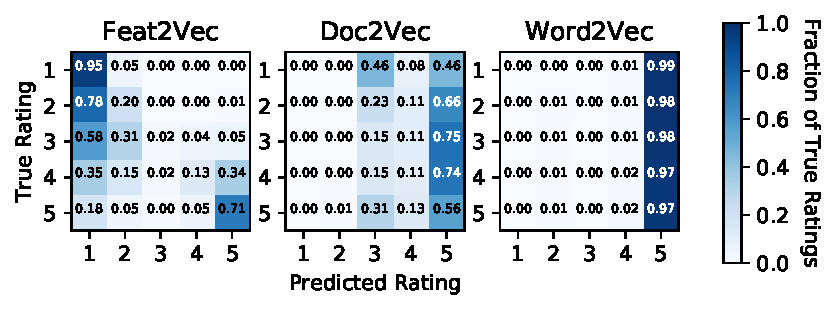
\includegraphics[width=.5\textwidth]{../paper/output/yelp/text_rating_confusionmat_numbers}
 \caption{Confusion Matrices of Self-Supervised Yelp Ratings Predictions}
 \label{fig:confmat}
 \end{figure}


\section{Conclusion}

Embeddings have proven useful in a wide variety of contexts, but they are typically built from datasets with a single feature type as in the case of Word2Vec, or tuned for a single prediction task as in the case of Factorization Machine.
We believe $\Feat2Vec$ is an important step towards general-purpose embedding methods.
It decouples feature extraction from prediction for datasets with multiple feature types,  it can be self-supervised, and its embeddings are easily interpretable.

In the supervised setting,  $\Feat2Vec$ outperforms an algorithm specifically designed for text---even when using the same feature extraction CNN.
In the self-supervised setting, $\Feat2Vec$ exploits the structure of a dataset to learn embeddings in a more sensible way than existing methods. This yields performance improvements in our ranking and prediction tasks.
To the extent of our knowledge, self-supervised $\Feat2Vec$  is the first method to calculate continuous representations of data with multi-modal feature types and no explicit labels.

Future work could study how to reduce the amount of  human knowledge our approach requires;
for example by automatically grouping features into entities, or by automatically choosing a feature extraction function.
These ideas can extend to our codebase that we make available
\footnote{The $\Feat2Vec$ model code is available  here: \url{https://www.dropbox.com/sh/wdr2sgt0z9gj6kb/AABlzw7QhteTYViSoMk3CDZpa?dl=0}. The self-supervised experiments using non-proprietary data are available here: \url{https://www.dropbox.com/sh/uc07ng403i4ss9a/AAAPshFzdOug_ooeLn4SGR3Ua?dl=0}{here}. The supervised experiments are available here: \url{https://goo.gl/zEQBiA}.
}.
Though further experimentation is necessary, we believe that our results are an encouraging step forward towards general-purpose embedding models.


{
\footnotesize
\footnotesize
\bibliographystyle{aaai}
\bibliography{joseg}
}




\end{document}
